\noindent

\includegraphics[height=1.25cm]{images/pictograms/replication}
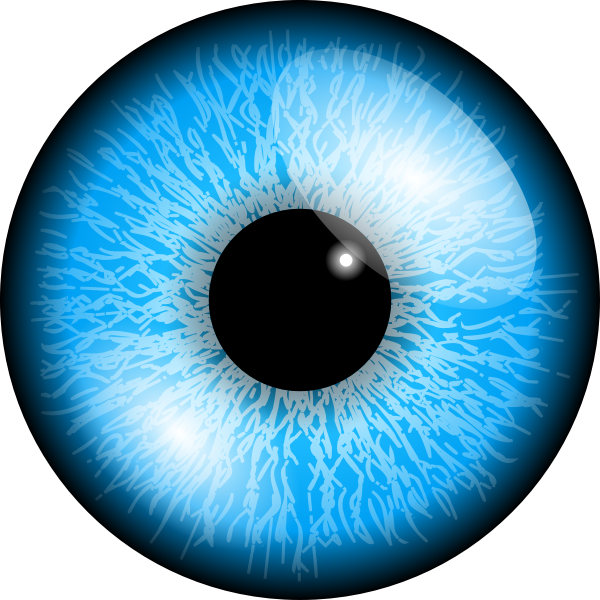
\includegraphics[height=1.25cm]{images/pictograms/visualisation}

\includegraphics[height=1.25cm]{images/pictograms/benchmark}

\includegraphics[height=1.25cm]{images/pictograms/under_construction}

\includegraphics[height=1.25cm]{images/pictograms/tools}

\includegraphics[height=1.25cm]{images/pictograms/FEM}

\includegraphics[height=1.25cm]{images/pictograms/FDM}

\includegraphics[height=1.25cm]{images/pictograms/3d}

\includegraphics[height=1.25cm]{images/pictograms/nonlinear}

\includegraphics[height=1.25cm]{images/pictograms/paraview}

%%%%%%%%%%%%%%%%%%%%%%%%%%%%%%%%%%%%%%%%%%%%%%%%%%%%%%%%%%%%%%%%%%%%%%%%%%%%%%%%%%%%%%%%%%%%%%%%%%%

\begin{flushright} {\tiny {\color{gray} python\_codes/fieldstone\_171/text.tex}} \end{flushright}

%\lstinputlisting[language=bash,basicstyle=\small]{python_codes/template_keywords.key}

\par\noindent\rule{\textwidth}{0.4pt}

\begin{center}
\inpython
{\small Code: \url{https://github.com/cedrict/fieldstone/tree/master/python_codes/fieldstone_171}}
\end{center}

\par\noindent\rule{\textwidth}{0.4pt}

{\sl This stone was developed in collaboration with L. van de Wiel}. \index{contributors}{L. van de Wiel}

\par\noindent\rule{\textwidth}{0.4pt}

Last revision: March. 23th, 2025.

\par\noindent\rule{\textwidth}{0.4pt}

%%%%%%%%%%%%%%%%%%%%%%%%%%%%%%%%%%%%%%%%%%%%%%%%%%%%%%%%%%%%%%%%%%%%%%%%%%%%%%%%%%%%%%%%%%%%%%%%%%%

There is a lot of literature and online material about these equations. Please consult them 
for reference:
\begin{itemize}
\item \fullcite{grsc84}
\item \fullcite{pear93}
\item \fullcite{muna14}
\item \url{http://www.mrob.com/pub/comp/xmorphia/index.html} by R. Munafo
\item \url{https://en.wikipedia.org/wiki/Reaction-diffusion_system}
\end{itemize}

The Gray–Scott reaction–diffusion system of equations are given by
\begin{eqnarray}
\frac{\partial U}{\partial t} &=& D_u \vec\nabla^2 U - UV^2 + F(1-U) \nn\\
\frac{\partial V}{\partial t} &=& D_v \vec\nabla^2 V + UV^2 - (F+k)V 
\end{eqnarray}
where $D_u$ and $D_v$ are diffusion coefficients associated with the species concentration $U$and $V$
$k$ is the dimensionless rate constant of the second reaction (also commonly called the `kill 
parameter') and $F$ is the dimensionless feed rate.
Often periodic boundary conditions are used. 

\textcite{gama23} (2023) rely on these equations to generate porous geometries 
and the following values of $D_u,D_v,f,k$ are used:

\begin{center}
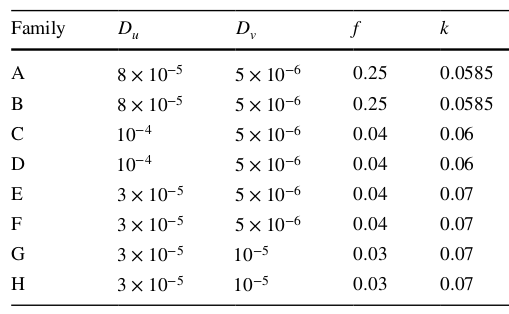
\includegraphics[width=6cm]{python_codes/fieldstone_171/images/gama01}
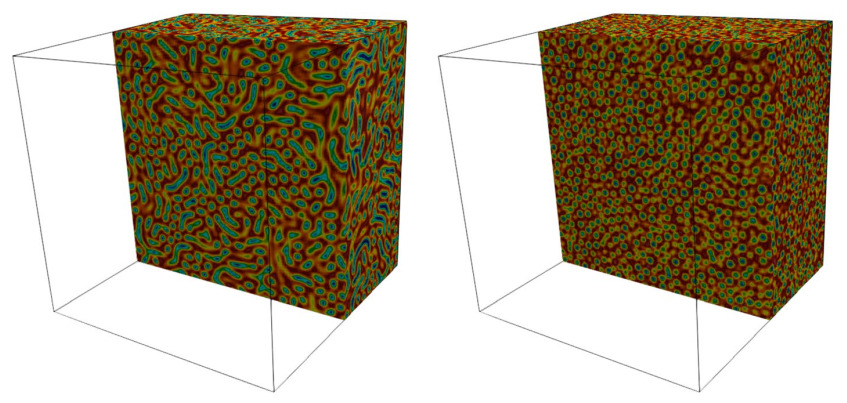
\includegraphics[width=9cm]{python_codes/fieldstone_171/images/gama02}\\
{\captionfont Iso-surfaces for solutions to the reaction-diffusion system 
for two set of parameters $\{D_u,D_v,F,k\}$, the parameters on the figure on 
the left(right) correspond to family A/B(C/D) in the table. The solutions were
obtained on a cube of length $L=192$.}
\end{center}

In the articles the authors use spherical initial distributions given by:
\begin{eqnarray}
U(r,\theta,\phi) &=& H_e(r-r_c) +\frac12 (1-H_e(r-r_c)) + 0.01 \cdot {\cal U}_{[0,1]} \nn\\
V(r,\theta,\phi) &=& \frac14 (1-H_e(r-r_c)) + 0.01 \cdot {\cal U}_{[0,1]}
\end{eqnarray}
where $H_e$ is the Heaviside step function, ${\cal U}_{[0,1]}$ is a random variable sourced from a 
uniform distribution defined between $[0,1]$, and $(r,\theta,\phi)$ are spherical coordinates centered at
the cube center, and $r_c$ is a constant (5 or 7).
The equations are solved numerically via a finite difference scheme on a cube of size $L$
with periodic boundary conditions. As time evolves, the patterns generated by
the solutions reveal a class of solutions whose iso-surfaces are reminiscent of the internal
boundaries encountered on porous media as shown in the figure above.



\textcite{pear93} (1993) reveals a surprising variety of irregular spatiotemporal patterns
as shown in Fig. 2\&3 of the paper:

\begin{center}
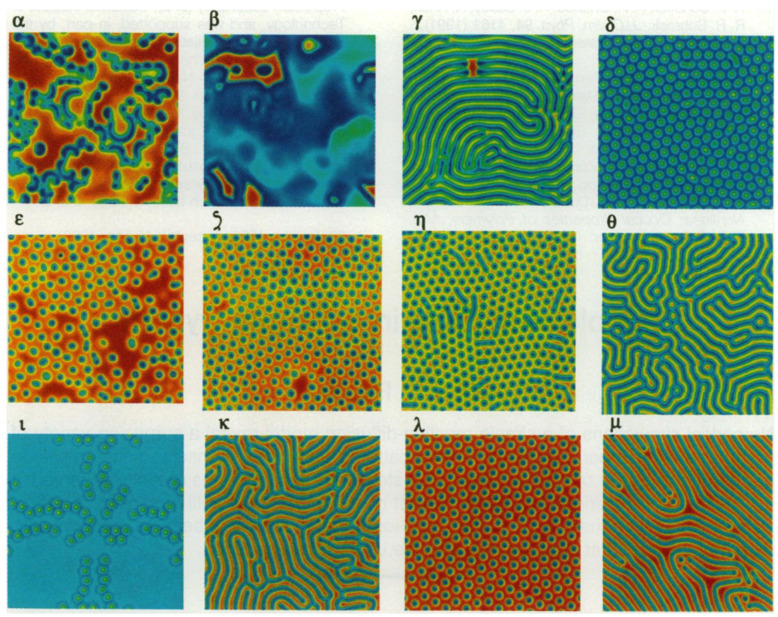
\includegraphics[height=7.5cm]{python_codes/fieldstone_171/images/pear93a}
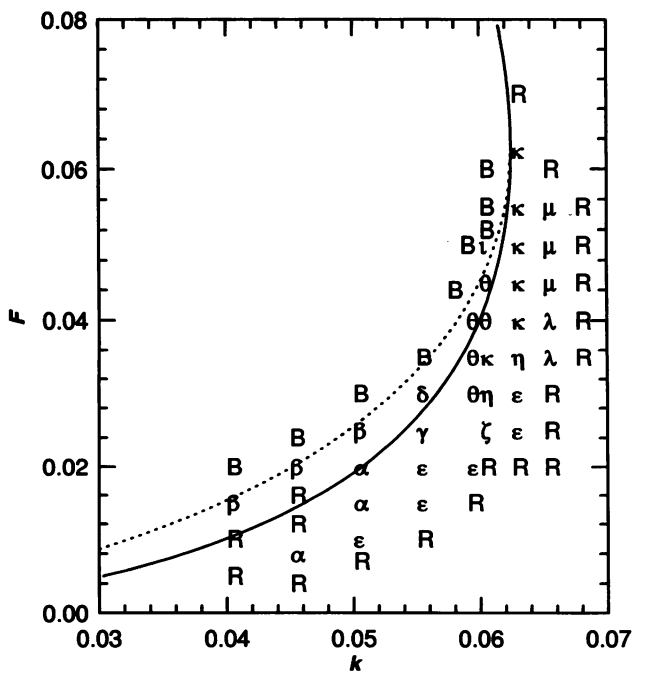
\includegraphics[height=7.5cm]{python_codes/fieldstone_171/images/pear93b}\\
{\captionfont Taken from \cite{pear93}. Left: The key to the map. The patterns 
shown in the figure are designated by Greek letters, which are used in 
[the right figure] to indicate the pattern found at a given point in parameter space.
Right: The Greek letters indicate the location in parameter
space where the patterns in [the left figure] were found; B and R indicate that
the system evolved to uniform blue and red states, respectively.
} 
\end{center}

In the paper the domain is a square of size $L=2.5$ with $D_u=2\cdot 10^{-5}$
and $D_v=10^{-5}$. The boundary conditions are periodic.
The simulations are forward Euler integrations of the finite-difference equations 
resulting from discretization of the diffusion operator. The spatial mesh consists of 256 by 256
grid points. The time step used is 1. Spot checks made with meshes as large as 1024 by
1024 and time steps as small as 0.01 produced no qualitative difference in the results.

Initially, the entire system was placed in the trivial state (U = 1,V = 0). The 20 by
20 mesh point area located symmetrically about the center of the grid was then
perturbed to (U = 1/2,V = 1/4). These conditions were then perturbed with $\pm 1\%$
random noise in order to break the square symmetry. The system was then integrated
for 200,000 time steps and an image was
saved. In all cases, the initial disturbance
propagated outward from the central
square, leaving patterns in its wake, until
the entire grid was affected by the initial
square perturbation. The propagation was
wave-like, with the leading edge of the
perturbation moving with an approximately
constant velocity. Depending on the param-
eter values, it took on the order of 10,000 to
20,000 time steps for the initial perturbation
to spread over the entire grid. The propagation velocity of the initial perturbation is
thus on the order of $1\cdot 10^{-4}$ space units per time unit. After the initial period during
which the perturbation spread, the system
went into an asymptotic state that was either
time-independent or time-dependent, depending on the parameter values.

Likewise in \textcite{gane22} (2022) we find the following figure:
\begin{center}
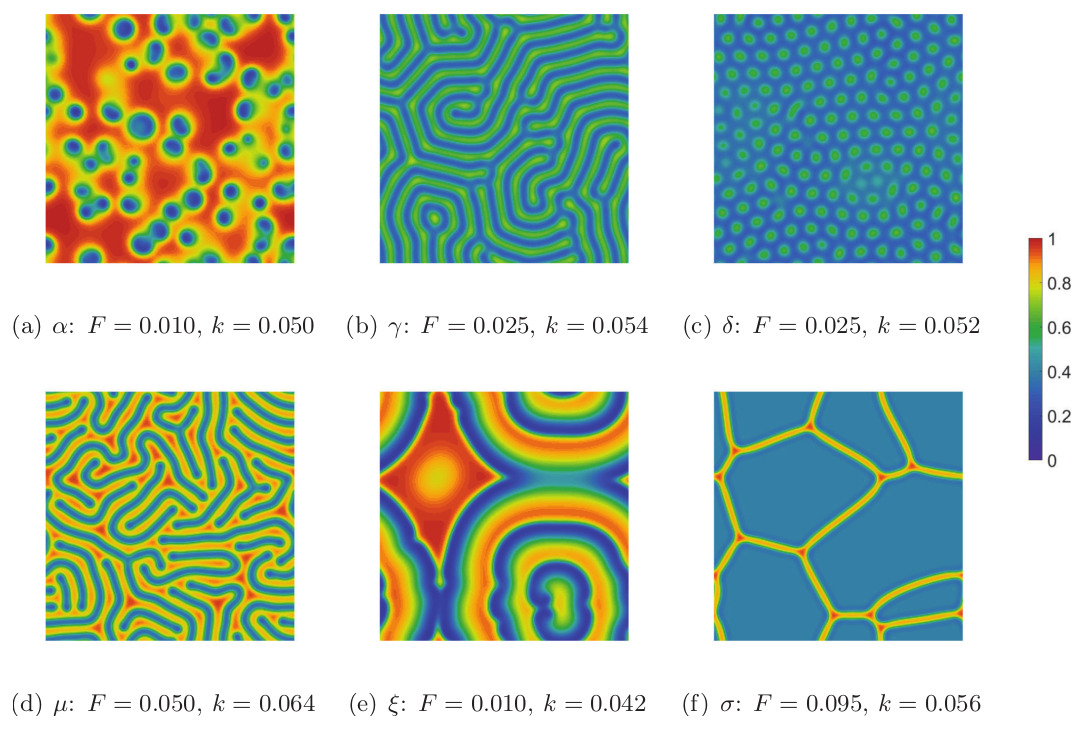
\includegraphics[height=7.5cm]{python_codes/fieldstone_171/images/gane22}\\
{\captionfont Taken from \cite{gane22}. 
Snapshots of a selection of two-dimensional patterns obtained for
$D_u=2\cdot 10^{-5}$ and $D_v=1\cdot 10^{-5}$ obtained via numerical 
simulation in MATLAB. (Code online.) Patterns
are classified according to the Greek letter naming convention used by \textcite{pear93}.
} 
\end{center}

%%%%%%%%%%%%%%%%%%%%%%%%%%%%%%%%%%%%%%%%%%%%%%%%%%%%
\section*{About the work of R. Munafo}

We find there\footnote{\url{http://www.mrob.com/pub/comp/xmorphia/pearson-classes.html}}
two key figures:

\begin{center}
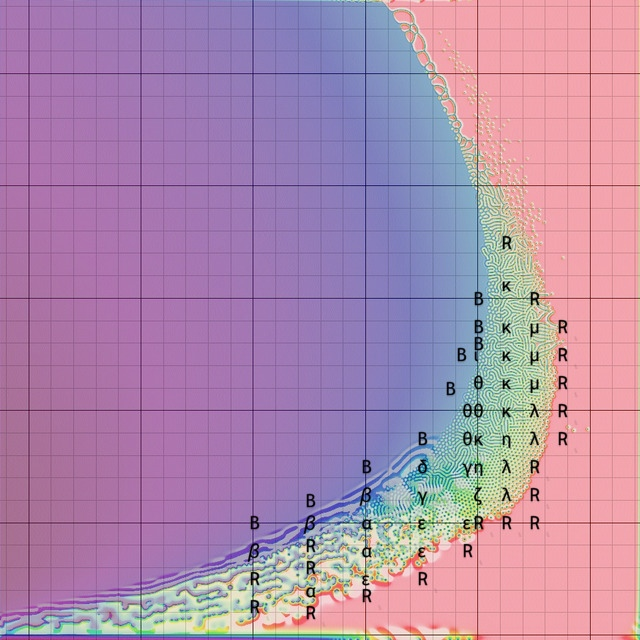
\includegraphics[height=7.5cm]{python_codes/fieldstone_171/images/pearson-orig}
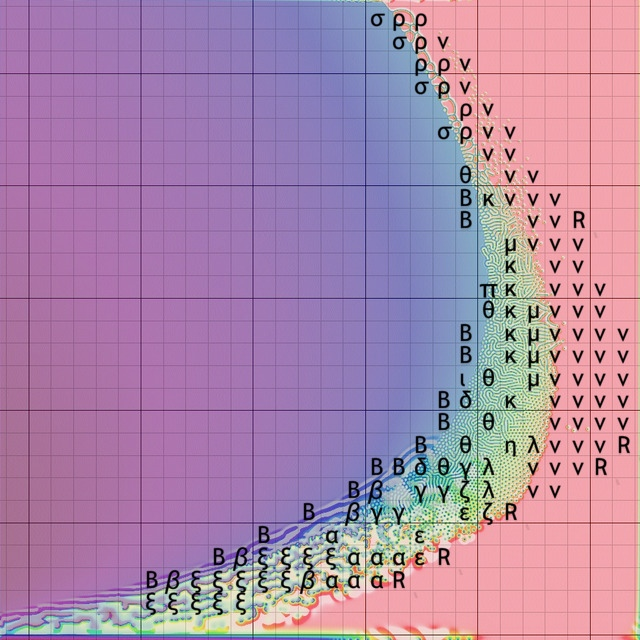
\includegraphics[height=7.5cm]{python_codes/fieldstone_171/images/pearson-tags}\\
{\captionfont So called key maps of the Gray-Scott equations. $k$ is on the 
horizontal axis, $F$ is on the vertical axis. Thick lines correspond to 
0.3-0.7 on the x-axis and to 0.3-0.8 on the y-axis.
The classification of the solution is traditionally based on Greek letters:
alpha ($\alpha$),    beta ($\beta$),    gamma ($\gamma$),    delta ($\delta$),    
epsilon ($\epsilon$),    zeta ($\zeta$),    eta ($\eta$),    
theta ($\theta$),    iota ($\iota$),    kappa ($\kappa$),    lambda ($\lambda$),    
mu ($\mu$),    nu ($\nu$),    xi ($\xi$),    pi ($\pi$),    rho ($\rho$),    sigma ($\sigma$).
The first fourteen
(R, B, and $alpha$ through $\mu$) were defined by Pearson \cite{pear93} (left figure); 
On the right we find the data from his figure 3 (with corrections) replotted on the index image from the left figure. 
}
\end{center}

The author states:
\begin{displayquote}
{\color{darkgray}
Pearson missed many types of patterns because he only used one starting pattern: 
a small (u, v) = (1/2, 1/4) square on an otherwise (1, 0) background. Many combinations of paramters (F, k) fail to produce 
a pattern if initialised this way, but produce patterns when started some other way (such as a single small spot on 
an otherwise (0, 1) background, resembling the inverse of Pearson's initialisation; or several spots of
diverse (F, k) values). Types nu, xi, pi, rho, and sigma are of this sort and were identified by me; 
the first three of these are described in my paper [2]. Types rho, and sigma also require a model with somewhat higher 
resolution than Pearson's, and significantly better runtime; these requirements would have made their discovery 
nearly impossible in the 1990s.
}
\end{displayquote} 



The classification is then as follows:
\begin{center}
\begin{tabular}{lll}
alpha   & (F=0.010, k=0.047) (F=0.014, k=0.053) \\
beta    & (F=0.014, k=0.039) (F=0.026, k=0.051) \\
gamma   & (F=0.022, k=0.051) (F=0.026, k=0.055) \\
delta   & (F=0.030, k=0.055) (F=0.042, k=0.059) \\
epsilon & (F=0.018, k=0.055) (F=0.022, k=0.059) \\
zeta    & (F=0.022, k=0.061) (F=0.026, k=0.059) \\
eta     & (F=0.034, k=0.063) 	\\
theta   & (F=0.030, k=0.057) (F=0.038, k=0.061) \\
iota    & (F=0.046, k=0.0594)   \\
kappa   & (F=0.050, k=0.063) (F=0.058, k=0.063) \\
lambda  & (F=0.026, k=0.061) (F=0.034, k=0.065) \\
mu      & (F=0.046, k=0.065) (F=0.058, k=0.065) \\
nu      & (F=0.054, k=0.067) (F=0.082, k=0.063) \\
xi      & (F=0.010, k=0.041) (F=0.014, k=0.047) \\
pi      & (F=0.062, k=0.061) \\
rho     & (F=0.090, k=0.059) (F=0.102, k=0.055) \\
sigma   & (F=0.090, k=0.057) (F=0.110, k=0.0523)
\end{tabular}
\end{center}






%%%%%%%%%%%%%%%%%%%%%%%%%%%%%%%%%%%%%%%%%%%%%%%
\section*{Lukas van de Wiel's approach}

In a private communication Lukas wrote:
{\small 
\begin{verbatim}
I used a resolution of 4800x4800 but 1000x1000 will most likely get you fine results.
The equations are:
dudt = DU * Lu +  FEED * (1.0 - u) - u*v^2
dvdt = DV * Lv - (FEED + KILL)* v  + u*v^2
with Lu and Lv the Laplacian of u and v.
For the pumice mesh: DU=0.000004, DV=0.000002, FEED=0.035, KILL=0.0575
Initial conditions:
u = 1, with random seed squares of a random size (edge length) 
between 11 and 60 and a value between 0.5 and 1
v = 0, with random seed squares of a random size (edge length) 
between 11 and 60 and a value between 0 and 0.25
The squares in u and those in v are independent from each other
I applied a thousand of these seeds in u and a thousand in v.
Time stepping: I use RK4 timesteps, with DT=0.001
Adaptive timestepping will probably be an improvement near the end,  
because the sharp edges around the seed squares will have gone.
It could no doubt be improved by turning the hard edges seed squares into 
soft edges seed blobs/gaussians, but then the smoothness of the patterns
depends on the parameters of Du and Dv, and needed something that works 
universally, for consistency. (If you reduce Du and Dv, you well get a more 
fine grained pattern, as if zoomed out more) 
Method of lines - no particular attention to nonlinearities. 
\end{verbatim}
}

\begin{center}
\includegraphics[width=5.6cm]{python_codes/fieldstone_171/images/u000000.jpg}
\includegraphics[width=5.6cm]{python_codes/fieldstone_171/images/u000001.jpg}
\includegraphics[width=5.6cm]{python_codes/fieldstone_171/images/u000003.jpg}\\
\includegraphics[width=5.6cm]{python_codes/fieldstone_171/images/u000007.jpg}
\includegraphics[width=5.6cm]{python_codes/fieldstone_171/images/u000012.jpg}
\includegraphics[width=5.6cm]{python_codes/fieldstone_171/images/u000020.jpg}\\
{\captionfont Solved in on a GPU, which did this in about a day, on 4800x4800.}
\end{center}

%%%%%%%%%%%%%%%%%%%%%%%%%%%%%%%%%%%%%%%%%%%%%%%%%%%%%%%%%%%%%%%%%%%%%%%%%%%%%%%%%%%%%
\section*{A word about methods}

The domain is a cuboid of size $L_x \times L_y \times L_z$.
It is discretised by means of a $nnx \times nny \times nnz = NP$ grid.

We are dealing with a set of coupled nonlinear PDEs to which there are no analytical solution.
We must then solve them by means of a numerical method. 
Obviously a Finite Difference of Finite Element approach could be envisaged. The main difficulty then
would be (as discussed in \stone~130) how to deal with the nonlinear terms. Also, based on 
the results presented above by Lukas it appears that a high resolution should be envisaged
of (at least?) $1000\times 1000$ nodes. This would yield *very* large linear systems to be 
solved hundreds/thousands of time.
Keeping this in mind we therefore decide to resort to the method of lines as in \stone~157.

We discretise the Laplace operators as follows:
\[
\vec\nabla^2 u \simeq 
\frac{u_{i-1,j,k}-2u_{i,j,k}+u_{i+1,j,k}}{h_x^2} + 
\frac{u_{i,j-1,k}-2u_{i,j,k}+u_{i,j+1,k}}{h_y^2} + 
\frac{u_{i,j,k-1}-2u_{i,j,k}+u_{i,j,k+1}}{h_z^2} 
\]
so that the PDEs can be discretised in space at a node $i$ as follows:
\begin{eqnarray}
\frac{\partial u_{i,j,k}}{\partial t} 
&=& D_u 
\left(
\frac{u_{i-1,j,k}-2u_{i,j,k}+u_{i+1,j,k}}{h_x^2} + 
\frac{u_{i,j-1,k}-2u_{i,j,k}+u_{i,j+1,k}}{h_y^2} + 
\frac{u_{i,j,k-1}-2u_{i,j,k}+u_{i,j,k+1}}{h_z^2} 
\right) \nn\\
&&- u_{i,j,k}v_{i,j,k}^2 + F(1-u_{i,j,k}) 
\nn\\
\frac{\partial v_{i,j,k}}{\partial t} &=& D_v 
\left(
\frac{v_{i-1,j,k}-2v_{i,j,k}+v_{i+1,j,k}}{h_x^2} + 
\frac{v_{i-1,j,k}-2v_{i,j,k}+v_{i+1,j,k}}{h_y^2} + 
\frac{v_{i,j,k-1}-2v_{i,j,k}+v_{i,j,k+1}}{h_z^2} 
\right) \nn\\
&&
+ u_{i,j,k}v_{i,j,k}^2 - (F+k)v_{i,j,k}
\end{eqnarray}

We then define $\vec{X}$ that is such that 
\[
\vec{X} = 
\left(
\begin{array}{c}
\vec{U} \\ \vec{V}
\end{array}
\right)
\] 
where $\vec{U}$ is the vector of all nodal $u$ values and 
$\vec{V}$ is the vector of all nodal $v$ values.

The equations above can then be written 
\[
\frac{d\vec{X}}{dt} 
= {\cal F} (\vec{X})
\]
The right-hand side of this equation is then implemented as follows:
\begin{lstlisting}
def F(Du,Dv,F,K,NP,hx,hy,hz,u,v):
    dX_dt=np.zeros(2*NP,dtype=np.float64)
    ...
    counter=0
    for i in range(0,nnx):
        for j in range(0,nny):
            for k in range(0,nnz):
                ...
                dX_dt[counter]=Duhx2*(u[front]-2*u[counter]+u[back])\
                              +Duhy2*(u[left] -2*u[counter]+u[right])\
                              +Duhz2*(u[top]  -2*u[counter]+u[bottom])\
                              -u[counter]*v[counter]**2+F*(1-u[counter])

                dX_dt[counter+NP]=Dvhx2*(v[front]-2*v[counter]+v[back])\
                                 +Dvhy2*(v[left] -2*v[counter]+v[right])\
                                 +Dvhz2*(v[top]  -2*v[counter]+v[bottom])\
                                 +u[counter]*v[counter]**2-(F+K)*v[counter]
                counter+=1
    ...
    return dX_dt
\end{lstlisting}
Note that the code above is not complete and only serves as an 
illustration of the struture of the function.

For simplicity the time derivative is discretised by means of a 1st-order
explicit approach, i.e.
\[
\frac{\vec{X}^{n+1} -\vec{X}^{n} }{\delta t} = {\cal F} (\vec{X}^n)
\]
or, 
\[
\vec{X}^{n+1}
=
\vec{X}^{n} + {\cal F} (\vec{X}^n) \delta t
\]
which translates into
\begin{lstlisting}
for istep in range(0,nstep+1):
    X[:]+=F(Du,Dv,Feed,Kill,NP,hx,hy,hz,u,v)*dt
    u[:]=X[0:NP]
    v[:]=X[NP:2*NP]
\end{lstlisting}
Periodic boundary conditions are implemented.

The solution vectors $\vec{U}$ and $\vec{V}$ are then exported to 
a vtu file every so often (controlled by the \lstinline{every} parameter).

At the moment the timestep is set to 0.1

Describe initial condition!

Write about njit

\newpage
%%%%%%%%%%%%%%%%%%%%%%%%%%%%%%%%%%%%%%%%%%%%%
\section*{Results}

\begin{center}
\includegraphics[width=10cm]{python_codes/fieldstone_171/results/stats}
{\captionfont opla}
\end{center}

\begin{center}
\includegraphics[width=5.6cm]{python_codes/fieldstone_171/results/u.0002.png}
\includegraphics[width=5.6cm]{python_codes/fieldstone_171/results/u.0022.png}
\includegraphics[width=5.6cm]{python_codes/fieldstone_171/results/u.0060.png}\\
\includegraphics[width=5.6cm]{python_codes/fieldstone_171/results/u.0100.png}
\includegraphics[width=5.6cm]{python_codes/fieldstone_171/results/u.0200.png}
\includegraphics[width=5.6cm]{python_codes/fieldstone_171/results/u.0300.png}\\
\includegraphics[width=5.6cm]{python_codes/fieldstone_171/results/u.0400.png}
\includegraphics[width=5.6cm]{python_codes/fieldstone_171/results/u.0500.png}
\includegraphics[width=5.6cm]{python_codes/fieldstone_171/results/u.0600.png}\\
{\captionfont opla}
\end{center}










\url{
http://www.mrob.com/pub/comp/xmorphia/ogl/index.html
}


\begin{verbatim}
And if you cannot get enough, there are the Brusselator equations, which are similar to Gray Scott but different:
dudt[idx] = DU * Lu[idx] + FEED - (KILL+1) * u[idx] + u[idx]*u[idx]*v[idx];
dvdt[idx] = DV * Lv[idx] +         KILL    * u[idx] - u[idx]*u[idx]*v[idx];
which have different pattern formations
(idx appears to indicate a 1D solution, but is actually 2D)
In general, while GS tend to have smooth shapes, B can have sharp wave fronts.
See section 1.1.1 of https://astro.pas.rochester.edu/~aquillen/phy411/Turing.pdf  for initial conditions.
\end{verbatim}




